% ----------------------------------------------------------------
% AMS-LaTeX Paper ************************************************
% **** -----------------------------------------------------------
\documentclass[11pt]{amsart}
\usepackage{graphicx, mathabx, amssymb,amsfonts,amsmath,amsthm,newlfont}
\usepackage{epsfig,url}
\usepackage{enumerate,enumitem}
\usepackage[colorlinks=true,linkcolor=red,citecolor=blue]{hyperref}
\usepackage[dvipsnames]{xcolor}
\usepackage{color}


%Clever ref
\usepackage[noabbrev,capitalize]{cleveref}

\usepackage[all,2cell]{xy} \UseAllTwocells \SilentMatrices

\usepackage{pstricks,pst-node,pst-tree}


%MARGINS

\setlength{\textwidth}{\paperwidth}
\addtolength{\textwidth}{-2.5in}
\calclayout

% ----------------------------------------------------------------
\vfuzz2pt % Don't report over-full v-boxes if over-edge is small
\hfuzz2pt % Don't report over-full h-boxes if over-edge is small
% THEOREMS -------------------------------------------------------
\newtheorem{thm}{Theorem}[section]
\newtheorem{corollary}[thm]{Corollary}
\newtheorem{lemma}[thm]{Lemma}
\newtheorem{proposition}[thm]{Proposition}
\newtheorem{Questions}[thm]{Questions}
\theoremstyle{definition}
\newtheorem{definition}[thm]{Definition}

\newtheorem{conjecture}{Conjecture} 
\newtheorem{QQ}{Question} 
\newtheorem{prob}{Problem}
\newtheorem{ex}[thm]{Examples}
\newtheorem{example}[thm]{Example}
\newtheorem{policy}{Policy}
\theoremstyle{remark}
\newtheorem{rem}[thm]{Remark}
\newtheorem{caveat}[thm]{Caveat}
\numberwithin{equation}{section}
% MATH -----------------------------------------------------------
\newcommand{\norm}[1]{\left\Vert#1\right\Vert}
\newcommand{\abs}[1]{\left\vert#1\right\vert}
\newcommand{\set}[1]{\left\{#1\right\}}

\newcommand{\To}{\longrightarrow}
\newcommand*{\Longhookrightarrow}{\ensuremath{\lhook\joinrel\relbar\joinrel\rightarrow}}
\newcommand{\Z}{\mathbb Z}
\newcommand{\Q}{\mathbb Q}
\newcommand{\C}{\mathbb C}
\newcommand{\Ok}{\mathcal O}
\newcommand{\ai}{\mathfrak{a}}
\newcommand{\bi}{\mathfrak{b}}
\newcommand{\R}{\mathbb R}
\newcommand{\N}{\mathbb N}
\newcommand{\AM}{A}
\newcommand{\xx}{\mathsf{x}}
\newcommand{\eqv}{\mathrm{ev}}
\font \rus= wncyr10
\newcommand{\sha}{\, \hbox{\rus x} \,}

\newcommand{\ari}{\mathrm{ar}} %arity
\newcommand{\obj}{\mathrm{Ob}} %object

\newcommand{\GC}{\mathcal{GC}}
\newcommand{\q}{/\!/}

\newcommand{\tr}{\mathrm{tr}}
\newcommand{\id}{\mathrm{id}}

\newcommand{\can}{\mathrm{can}}

\newcommand{\mm}{\mathfrak{m}}

\newcommand{\GL}{\mathrm{GL}}
\newcommand{\LP}{L}
\newcommand{\FL}{F\!L}
\newcommand{\mc}{\mu}

\newcommand{\0}{\color{blue}{\mathsf{0}}}

%%%%Macros PL
\newcommand{\Alt}{ \mid\!\!\mid  } 
\newcommand{\inc}{\subseteq}
 \newcommand{\incs}{\subsetneq}
\newcommand{\union}{\cup}
\newcommand{\Union}{\bigcup}	
\newcommand{\comp}{\circ}
\newcommand{\setc}[2]{\set{#1 \mid #2}}

\newcommand \seq[2]{\shortstack{$#1$ \\ \mbox{}\\
                    \mbox{}\hrulefill\mbox{}\\ \mbox{}\\ $#2$}}
\newcommand{\cat}[1]{{\mathbb #1}}
\newcommand{\dl}{[\![} 			
\newcommand{\dr}{]\!]} 
\newcommand{\hyper}[1]{{\mathbb #1}}	
\newcommand{\restrH}[2]{\hyper{#1}\backslash #2}

%Operades

\def\calO{\mathcal{O}}
\newcommand{\KK}{\mathbb{K}}
\newcommand{\opd}[1]{\mathcal{#1}}

%Antischrieck
\newcommand{\as}{{\scriptstyle \text{\rm !`}}}

%Definitions
\definecolor{darkblue}{rgb}{0,0,0.7} % darkblue color
\newcommand{\darkblue}{\color{darkblue}} % darkblue command
\newcommand{\defn}[1]{{\darkblue \emph{#1}}}

%Commentaires 

\newcommand{\Guillaume}[1]{\textcolor{magenta}{\underline{Guillaume}: #1}}
\newcommand{\correction}[1]{\textcolor{red}{#1}}

%Source and sink
\newcommand{\so}{\mathrm{sc}} 
\newcommand{\sk}{\mathrm{sk}} 


\newcommand{\op}{\mathrm{op}}

%PL
\newcommand{\occ}[2]{#1/#2}
\newcommand{\recrestr}[2]{#1_{\cap #2}}
\newcommand{\xyz}[3]{#1\stackrel{#2}{\rightsquigarrow}#3}

\newcommand{\PL}[1]{{\color{red}{#1}}}

\newcommand{\calP}{\mathcal{P}}
\newcommand{\calH}{\mathcal{H}}

%Operators
\DeclareMathOperator{\Sat}{Sat}
\DeclareMathOperator{\supp}{supp}
\DeclareMathOperator{\Ter}{Ter}
\DeclareMathOperator{\sort}{sort}
\DeclareMathOperator{\arisort}{arisort}
\DeclareMathOperator{\var}{var}

%Drapeau européen

\usepackage{graphicx,calc}
\newlength\myheight
\newlength\mydepth
\settototalheight\myheight{Xygp}
\settodepth\mydepth{Xygp}
\setlength\fboxsep{0pt}
\newcommand*\inlinegraphics[1]{%
  \settototalheight\myheight{Xygp}%
  \settodepth\mydepth{Xygp}%
  \raisebox{-\mydepth}{\includegraphics[height=\myheight]{#1}}%
}

%Dessins

\usepackage{tikz}
\usepackage{tikz-cd}
\usepackage{pgfplots}
\usepackage{pgfplotstable}
\tikzset{math3d/.style=
    {x= {(-0.353cm,-0.353cm)}, z={(0cm,1cm)},y={(1cm,0cm)}}}
\tikzset{JLL3d/.style=
    {x= {(0.4cm,-0.2cm)}, z={(0cm,1cm)},y={(-1cm,0cm)}}}
\usetikzlibrary{calc}
\usetikzlibrary{shapes,shapes.geometric,fit,positioning,calc,matrix}
\tikzset{
  optree/.style={scale=.5,thick,grow'=up,level distance=10mm,inner sep=1pt},
  comp/.style={draw=none,circle,fill,line width=0,inner sep=0pt},
  dot/.style={draw,circle,fill,inner sep=0pt,minimum width=3pt},
  circ/.style={draw,circle,inner sep=1pt,minimum width=4mm},
  emptycirc/.style={draw,circle,inner sep=1pt,minimum width=2mm},
  root/.style={level distance=10mm,inner sep=1pt},
  leaf/.style={draw=none,circle,fill,line width=0,inner sep=0pt},
  nodot/.style={draw,circle,inner sep=1pt},
}

\pgfplotsset{compat=1.12}





% ----------------------------------------------------------------

\def\abovespace{\vspace{12pt}}
\def\belowspace{\vspace{8pt}}



\addtolength{\hoffset}{-0.0in} \addtolength{\textwidth}{0in}
\addtolength{\voffset}{-0.0in} \addtolength{\textheight}{0.0in}


% -----------------------------------------------------------------

\title{Term rewriting on nestohedra}

\author{Pierre-Louis Curien}
\address{IRIF, Universit\'e Paris Diderot and $\pi r^2$ team, Inria, France.}
\email{curien@irif.fr}

\author{Guillaume Laplante-Anfossi}
\address{School of Mathematics and Statistics, University of Melbourne, Victoria, Australia.}
\email{guillaume.laplanteanfossi@unimelb.edu.au}

\date{\today}

\subjclass[2020]{Primary 18N20, Secondary 52B11?} 

\keywords{Term rewriting, nestohedra, hypergraph polytopes, categorified operads, categorical coherence, MacLane coherence theorem.}

\thanks{The second author was supported by the Australian Research Council Future Fellowship FT210100256 and the Andrew Sisson Fund.}


\begin{document}

\begin{abstract}
We define term rewriting systems on the vertices and faces of nestohedra, and show that the former are confluent. 
While the associated poset on vertices generalizes Barnard--McConville's flip order for graph-associahedra, the preorder on faces likely generalizes the facial weak order for permutahedra. 
Moreover, we define and study contextual families of nestohedra, whose local confluence diagrams satisfy a certain uniformity condition. 
The proof of confluence of their rewriting systems reproduce, via Huet's correspondence, categorical coherence theorems for monoidal categories, categorified permutads and operads.
\end{abstract}

\maketitle

\setcounter{tocdepth}{1}
%\tableofcontents

% !TEX root = ../Coherence2.tex

\section*{Introduction} 
\label{s:introduction}

TBC


\subsection*{Notations}

We use $\prec$ to denote cover relations in a poset, and $|-|$ to denote the cardinality of a set.
% !TEX root = ../Coherence2.tex

\section{Hypergraph polytopes} 
\label{s:hypergraph}

In this section, we recall the definition of hypergraph polytopes. 
We refer to \cite{DP-HP,COI} for more details. 

%%%%%%%%%%%%%%%%%%%%%%%%%%%%%%%%%%%%%%%%%%%

\subsection{Hypergraphs}
A \defn{hypergraph} is given by a finite set $H$ of \defn{vertices} and a subset of \defn{hyperedges} $\hyper{H}\inc {\cal P}(H)\setminus\emptyset$ such that $\Union \hyper{H}=H$. 
We always assume that $\hyper{H}$ is \defn{atomic}, that is $\set{x}\in \hyper{H}$, for all $x\in H$. 
A hyperedge of cardinality 2 is called an \defn{edge}.  
For $X\inc H$, the \defn{plain restriction} of $\hyper{H}$ to $X$ is the set 
$\hyper{H}_X := \setc{Z\in \hyper{H}}{\; Z\inc X}$.

We say that $\hyper{H}$ is \defn{connected} if there is no non-trivial partition $H=X_1\union X_2$ such that $\hyper{H}=\hyper{H}_{X_1}\union \hyper{H}_{X_2}$. 
For each hypergraph, there exists a partition $H=X_1\union\ldots\union X_m$ such that each $\hyper{H}_{X_i}$ is connected and $\hyper{H}=\Union(\hyper{H}_{X_i})$.  
The $\hyper{H}_{X_i}$'s are called the \defn{connected components} of $\hyper{H}$.
For $X\inc H$, we say that a non-empty subset $X$ of vertices is \defn{connected} (resp. a \defn{connected component}) whenever $\hyper{H}_X$ is connected (resp. a connected component of $\hyper{H}$).  
We denote by $\restrH{H}{X}:=\hyper{H}_{H\setminus X}$ the plain restriction of $\hyper{H}$ to $H \setminus X$.
The \defn{saturation} of $\hyper{H}$ is the hypergraph
$\Sat(\hyper{H})=\setc{X}{\emptyset\incs X\inc H\;\mbox{and}\;\hyper{H}_X\;\mbox{is connected}}$.
A hypergraph is called \defn{saturated} when $\hyper{H}=\Sat(\hyper{H})$.  
The \defn{reconnected restriction} of $\hyper{H}$ to $X$ is the set $$\recrestr{\hyper{H}}{X}:=\setc{Z\cap X}{Z\in \Sat(\hyper{H}), Z\cap X\neq\emptyset}.$$

\begin{rem}
    Atomic and saturated hypergraphs are called \defn{building sets} in the nestohedra literature, see for example \cite{P09,FS05}.
\end{rem}

For $X\inc H$, we will express the fact that $\setc{H_i}{i\in I}$ is the set of connected components of $\restrH{H}{X}$ by the notation $\hyper{H},X  \leadsto  \setc{H_i}{i\in I}.$
If $I=\set{1,\ldots,n}$, we write simply $\hyper{H},X  \leadsto H_1,\ldots,H_n$, with no order intended.
We will write $\hyper{H}_i$ for $\hyper{H}_{H_i}$.
In the specific situation where $x,y,z\in H$ and $\hyper{H},\set{x}\leadsto \setc{H_i}{i\in I}$, we shall write
$$\begin{array}{ll}
\xyz{x}{\hyper{H}}{\set{y,z}} & \mathrm{if}\; y,z\in H_i\; \mbox{for some}\; i \in I\\
\xyz{x}{\hyper{H}}{\set{y},\set{z}} & \mbox{otherwise}.
\end{array}$$
In the second case, we will say that $x$ \defn{disconnects} $y$ and $z$ in $\hyper{H}$. 
The reconnected restriction allows one to charaterize the preceding two situations as follows.

\begin{lemma} 
\label{xyz-reconnected} 
We have
$$\begin{array}{lll}
\xyz{x}{\hyper{H}}{\set{y,z}} & \mathrm{iff} & \recrestr{\hyper{H}}{\set{x,y,z}},\set{x}\leadsto\set{y,z} \\
\xyz{x}{\hyper{H}}{\set{y},\set{z}} & \mathrm{iff} & \recrestr{\hyper{H}}{\set{x,y,z}},\set{x}\leadsto \set{y},\set{z}.
\end{array}$$
\end{lemma}

\begin{proof} 
    Let $\hyper{H},x\leadsto H_1,\ldots,H_n$. 
    Suppose $\xyz{x}{\hyper{H}}{\set{y,z}}$. 
    Then there exists $i$ such that $\set{y,z}\inc H_i$, and hence $\set{y,z}\inc H_i\cap\set{x,y,z}$, and in fact $\set{y,z} = H_i\cap\set{x,y,z}$ since $x\not\in H_i$. 
    Thus $\recrestr{\hyper{H}}{\set{x,y,z}},\set{x}\leadsto\set{y,z}$ holds by definition of reconnected restriction.
    If $\xyz{x}{\hyper{H}}{\set{y},\set{z}}$, then there exist $i\neq j$ such that $y\in H_i$ and $z\in H_j$. 
    We then derive likewise $H_i\cap\set{x,y,z}=\set{y}$ and $H_j\cap\set{x,y,z}=\set{z}$ from which $ \recrestr{\hyper{H}}{\set{x,y,z}},\set{x}\leadsto \set{y},\set{z}$ follows.
\end{proof}

%%%%%%%%%%%%%%%%%%%%%%%%%%%%%%%%%%%%%%%%%%%%%%%%%%%%%%%

\subsection{Constructs}
A {connected} hypergraph $\hyper{H}$ gives rise to a set of \defn{constructs}, which are defined inductively as follows.
 
\begin{definition} 
\label{inductive-construct}
%as follows.
Let $\hyper{H}$ be a connected hypergraph and $Y$ be a non-empty subset of $H$.
\begin{enumerate}
\item  If $Y = H$, then the one-node tree $H$ decorated with $H$ is a construct of $\hyper{H}$.
\item If $\hyper{H},Y  \leadsto H_1,\ldots,H_n$, and if $T_1,\ldots,T_n$ are constructs of $\hyper{H}_1,\ldots,\hyper{H}_n$, respectively, then the
tree $Y(T_1,\ldots,T_n)$ whose root is decorated by $Y$, with $n$ outgoing edges on which the respective $T_i\,$'s are grafted is a construct.  
\end{enumerate}
When $Y={z}$ is a singleton, we freely write $z$ in place of $\set{z}$.
A \defn{construction} is a construct all of whose nodes are  decorated with singletons. 
\end{definition}

Since all decorations in a construct are disjoint, we freely identify nodes with subsets of $H$. 
We use the notation $\occ{T}{X}$ to denote the full subtree of $T$ rooted at $X$, defined only if $X$ is indeed a decoration of a node of $T$. 
If $S$ is a (not necessarily full) subtree of $T$, we denote by $\supp(S)$ the union of the decorations of the nodes of $S$.

\begin{rem} \label{subconstruct-restriction}
The intention behind this presentation is algorithmic: a construct is built by picking and removing a non-empty subset $Y$ of $H$, then branching to the connected components of $\restrH{H}{Y}$ and continuing inductively in all the branches.
It follows readily from the definition that $\occ{T}{X}$ is a construct of $\hyper{H}_{\supp(\occ{T}{X})}$.
\end{rem}

\begin{rem}
    The notion of construct is equivalent to the notion of nested set \cite{P09}, and to the notion of tubing in the case where $\hyper{H}$ is a graph~\cite{CD-CCGA}.  
    We refer to \cite[Sec.~3.1]{COI} for details.
\end{rem}

%Here we content ourselves with a sketchy description of the
%dictionary (for the readers familiar with nested sets).
%Given a construct $T$, take the set $\setc{\supp(\occ{T}{X})}{X\:\textrm{is a node of}\: T}$. Conversely, read a construct from a nested set $\mathbb{T}$ as follows: for each  $Z\in\mathbb{T}$, consider the elements $Z_1,\ldots, Z_n\in\mathbb{T}$ that are maximal among all elements of $\mathbb{T}$ that are strictly included in $Z$, then $Z\setminus\bigcup(Z_1\cup \ldots \cup Z_n)$ will decorate a node of the corresponding construct. 
%The subface relation formulated in terms of nested sets is just the inclusion of nested sets.

If $X,Y$ are two nodes of a construct $S$ of $\hyper{H}$, $X$ being the father of $Y$, we can define a new construct $T$ by contracting the edge between $X$ and $Y$, and labeling the resulting vertex of~$T$ by the union of the labels of $X$ and $Y$. 

\begin{definition}
    We denote $({\cal A}(\hyper{H}),\preceq)$ the poset of constructs of a connected hypergraph~$\hyper{H}$ obtained as the reflexive and transitive closure of the following covering relations: a construct $S$ covers a construct $T$ if $T$ can be obtained from $S$ by contracting an edge.
\end{definition}

%%%%%%%%%%%%%%%%%%%%%%%%%%%%%%%%%%%%%%%%%%%%%%

\subsection{Hypergraph polytopes}
\label{ss:hypergraph-polytopes}

We are now ready to define hypergraph polytopes, a.k.a nestohedra.

\begin{definition}
    A \defn{hypergraph polytope} is a polytope whose face lattice is isomorphic to the poset of constructs of some connected hypergraph $\hyper{H}$.
\end{definition}

Do\v sen and Petri\'c gave polytopal realisations of hypergraph polytopes in ~\cite{DP-HP}.
The idea is that the connected subsets of $\hyper{H}$ specify the faces of a fixed $(|H|-1)$-dimensional simplex, that are to be truncated according to the constructs of $\hyper{H}$.

Let us introduce a few families of hypergraph polytopes that will be studied in \cref{ss:examples}.
When $\hyper{H}$ is a graph, these are known as \emph{graph-associahedra} \cite{CD-CCGA}.

\subsubsection{Simplices}
The $n$-dimensional \defn{simplex} is the realization of the hypergraph 
$$\mathbb{S}_n:=\{\{x_1\},\{x_2\},\ldots,\{x_{n+1}\},\{x_1,\ldots,x_{n+1}\}\}.$$

\subsubsection{Cubes}
The $n$-dimensional \defn{cube} is the realization of the hypergraph
$$\mathbb{C}_n:=\{\{x_j \ | \ 1 \leq j \leq i \} \ | \ 1 \leq i \leq n+1\}.$$

\begin{rem}
  Note that these two families of hypergraph polytopes are defined by genuine hypergraphs, contrary to the following families of graph-associahedra.
\end{rem}

\subsubsection{Associahedra}
The $n$-dimensional \defn{associahedron} is the realization of the hypergraph 
$$\mathbb{K}_n:=\{\{x_1\},\{x_2\},\ldots,\{x_{n+1}\},\{x_1,x_2\},\ldots,\{x_n,x_{n+1}\}\}.$$
In other words, it is the graph-associahedron for the linear graph with $n+1$ vertices.

\subsubsection{Permutahedra}
The $n$-dimensional \defn{permutahedron} is the realization of the hypergraph 
$$\mathbb{P}_n:=\{\{x_1\},\{x_2\},\ldots,\{x_{n+1}\}\} \cup \{\{x_i,x_j\} \ | \ 1 \leq i \neq j \leq n+1 \}.$$
In other words, it is the graph-associahedron for the complete graph on $n+1$ vertices.

\begin{rem}
  Note that the definition of $\hyper{S}_n$ and $\hyper{P}_n$ does not depend on any order on the vertices, while the definition of $\hyper{C}_n$ and $\hyper{K}_n$ involves the total order on~$\set{1\ldots,n}$. 
\end{rem}

\subsubsection{Operahedra}
To every rooted planar tree $\calT$ with $n+2$ vertices, one can associate its $n$-dimensional \defn{operahedron}, whose faces are in bijection with nestings of $\calT$ \cite{laplante-anfossiDiagonalOperahedra2022a,CLA1}.
These are in bijections with the tubings of the \defn{line graph} $\mathbb{L}(\calT)$ of $\calT$.
The vertices of $\mathbb{L}(\calT)$ are the edges of ${\cal T}\!$, and two vertices are connected whenever as edges of ${\cal T}$ they share a common vertex, see \cref{fig:line-graph}.
In other words, an $n$-dimensional operahedron is the graph-associahedron for a clawfree block graph with $n+1$ vertices.

\begin{figure}[h!]
  \begin{center}
    \begin{tabular}{ccc}
    \resizebox{2cm}{!}{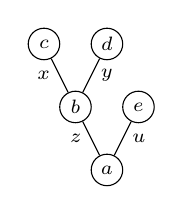
\begin{tikzpicture}[scale=0.8]
        % set up the nodes
        \node (E)[circle,draw=black,minimum size=4mm,inner sep=0.1mm] at (0,0) {\scriptsize $a$};
        \node (F) [circle,draw=black,minimum size=4mm,inner sep=0.1mm] at (-0.5,1) { \scriptsize $b$};
        \node (A) [circle,draw=black,minimum size=4mm,inner sep=0.1mm] at (0.5,1) {\scriptsize $e$};
        \node (Asubt) [circle,draw=black,minimum size=4mm,inner sep=0.1mm] at (-1,2) {\scriptsize  $c$};
        \node (P) [circle,draw=black,minimum size=4mm,inner sep=0.1mm] at (0,2) {\scriptsize $d$};
        % draw arrows and text between them
        \draw[-] (E)--(F) node  [midway,left] {\scriptsize $z$};
        \draw[-] (E)--(A) node  [midway,right] {\scriptsize $u$};
     \draw[-] (F)--(Asubt) node [midway,left] {\scriptsize $x$};
     \draw[-] (F)--(P) node [midway,right] {\scriptsize $y$};
       \end{tikzpicture}}
    
    &&
    \resizebox{2cm}{!}{
    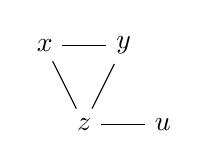
\begin{tikzpicture}
        % set up the nodes
        \node (Z)[] at (-0.5,0) {$z$};
        \node (U)[]  at (0.5,0) {$u$};
        \node (X)[]  at (-1,1) {$x$};
        \node (Y)[]  at (0,1) {$y$};
        % draw arrows and text between them
        \draw[-] (Z)--(U) node  {};
     \draw[-] (Z)--(X) node  {};
     \draw[-] (Z)--(Y) node {};
     \draw[-] (X)--(Y) node {};
       \end{tikzpicture}}
    \end{tabular}
    \end{center}
    \caption{A planar tree with $5$ vertices (left) and its line graph (right).}
    \label{fig:line-graph}
\end{figure}

Many more examples are to be found in~\cite{DP-HP,COI,CDOO}, as well as in the abundant literature on nestohedra.




% !TEX root = ../Coherence2.tex

\section{Dimensional faces} 
\label{s:2faces}

In this section, we describe the $2$-dimensional faces of hypergraph polytopes.

%%%%%%%%%%%%%%%%%%%%%%%%%%%%%%%%%%%%%%%%%%%

\subsection{Two types of $2$-faces}
woijew






% !TEX root = ../Coherence2.tex

\section{Hypergraphic rewrite systems} 
\label{s:rewriting}

We associate to each hypergraph a term rewrite system given by its constructs.

%%%%%%%%%%%%%%%%%%%%%%%%%%%%%%%%%%%%%%%

\subsection{Constructs as closed terms}

A \defn{signature} $\Sigma$ is a tuple $(V,F,S,\ari,\outsort,\insort)$ made of 
\begin{itemize}
  \item a set $V$ of \defn{variables},
  \item a non-empty set $F$ of \defn{function symbols}, and
  \item a set $S$ of \defn{sorts},
\end{itemize}
together with an \defn{arity}, \defn{output sort} and \defn{input sort} functions
\begin{itemize}
  \item $\ari : F \to \mathbb{N}$,
  \item $\outsort : F \cup V \to S$,
  \item $\insort : F \to \Sigma_{n \geq 0} S^{n}$,
\end{itemize}
such that for $f \in F$, we have $\insort(f) \in S^{\ari(f)}$. 
The $i$th component of $\insort(f)$ is denoted $\insort(f,i)$.
The set $\Ter(\Sigma)$ of \defn{terms} over a signature $\Sigma$ is defined inductively as follows. 
\begin{enumerate}
  \item If $t \in V$ is a variable, then $t$ is a term.
  \item If $f \in F$ is an arity $n$ function symbol, and $t_1,\ldots,t_n$ are terms such that $\outsort(t_i)=\insort(f,i)$, then $f(t_1,\ldots,t_n)$ is a term, and $\outsort(f(t_1,\ldots,t_n)):=\outsort(f)$.
\end{enumerate}
For a term $t \in \Ter(\Sigma)$, its set of \defn{variables} is defined as 
\begin{equation*}
  \var(t) := 
  \begin{cases}
    \{t\} & \text{ if } t \in V, \\
    \bigcup_{1 \leq i \leq n}\var(t_i) & \text{ if } t=f(t_1,\ldots,t_n).
  \end{cases}
\end{equation*}
A term $t$ is \defn{closed} if it does not contain any variable, i.e. if $\var(t)=\emptyset$.
A \defn{rewrite rule} over $\Sigma$ is an ordered pair $(l,r)$ of terms in $\Ter(\Sigma)$, denoted $l \to r$, such that
\begin{enumerate}
  \item the first term $l$ is not a variable, that is $l \notin V$.
  \item the variables of the second term are already in the first term, that is $\var(r) \subseteq \var(l)$.
\end{enumerate}

\begin{definition}
  A many-sorted \defn{term rewrite system} is a pair $(\Sigma,R)$ made of a signature and a set of rewrite rules $R$ over $\Sigma$.
\end{definition}

\begin{definition} \label{def:signature-hyper}
  Let $\hyper{H}$ be a connected hypergraph. 
Consider the signature $\Sigma_\hyper{H}$ made of the following data: 
\begin{itemize}
  \item Variables are connected subsets of $H$, that is $$V:=\{ X \subseteq H \ | \ \hyper{H}_{X} \text{ is connected}\}.$$ 
  \item Function symbols are pairs of a connected subset of $H$ and one of its subsets 
  $$F:=\{(X,Y) \ | \ X \subseteq Y \subseteq H, \ \hyper{H}_Y \text{ is connected}\}.$$
  \item Sorts are either the ``variable" sort, or a connected subset of $H$, i.e. 
  $$S:=\{ X \subseteq H \ | \ \hyper{H}_X \text{ is connected}\}.$$
  \item For $(X,Y) \in F$, we define $\ari(X,Y)$ as the number of connected components of $\hyper{H}_Y\setminus X$.
  \item Variables $X \in V$ are their own output sort $\outsort(X):=X$, while function symbols $(X,Y) \in F$ have output sort $\outsort(X,Y):=Y$.
  \item For function symbols $(X,Y) \in F$ such that $\hyper{H}_Y,X \leadsto Y_1,\ldots,Y_k$, and for $1 \leq i \leq k$, we define $\insort((X,Y),i):=Y_i$.
\end{itemize}
\end{definition}


\begin{lemma} \label{l:bijection-terms}
  There is a bijection between the set of closed terms of output sort $H$ over $\Sigma_\hyper{H}$ and the set of constructs of $\hyper{H}$.
\end{lemma}

\begin{proof}
  We compare the inductive definition of constructs (\cref{inductive-construct}) with the inductive definition of $\Ter(\Sigma_\hyper{H})$ above.
  First observe that there is only one closed term (arity $0$ function symbol) of output sort $H$, the pair $(H,H)$. 
  We associate to this term the tree with only one node, decorated by $H$.
  Now, an arity $n$ function symbol of type $H$ is a pair $(Y,H)$ with $Y \subseteq H$. 
  If $\hyper{H}_X,Y \leadsto H_1,\ldots,H_n$, then a valid closed term $(Y,H)(t_1,\ldots,t_n)$ is made of closed terms $t_i$ of type $H_i$, for $1 \leq i \leq n$. 
  This means that $t_i$ is of the form $(Y',H_i)(t_1',\ldots,t_k')$ for some subset $Y' \subseteq H_i$. 
  We associate to the term $(Y,H)(t_1,\ldots,t_n)$ the tree $Y(T_1,\ldots,T_n)$ with root decorated by $Y$, and the trees~$T_i$, associated by induction to the various $t_i$'s, grafted on its leaves.
  It is clear from the inductive nature of the definitions that this correspondence is bijective.
\end{proof}

Now suppose that the vertices of our hypergraph $\hyper{H}$ are equipped with a total ordering.
According to \cref{l:bijection-terms}, we can consider the consructs of $\hyper{H}$ as terms. 
Then, we can define a family of rewrite rules as follows.

\begin{definition} \label{def:rules}
  Let $\hyper{H}$ be a hypergraph. 
  Let $K$ be a connected subset of $H$, and let $X \subseteq K$ be such that $\mathbb{K},X \leadsto K_1,\ldots K_n$.
  Let $Y \subseteq K_i$ be a subset of a connected component $K_i$ for some $1 \leq i \leq n$, and suppose that $\mathbb{K}_i\setminus Y$ has $p$ connected components. 
  Then for $V_1,\ldots,V_n$ and $(V_i)^1,\ldots,(V_i)^p$ variables, we define 
  $$(X,K)(V_1,\ldots, V_{i-1},(Y,K_i)((V_i)^1,\ldots, (V_i)^p),V_{i+1},\ldots,V_n)$$
  $$ \longrightarrow (X\cup Y,K)(V_1,\ldots,V_{i-1},(V_i)^1,\ldots, (V_i)^p,V_{i+1},\ldots,V_n)$$
  if $\max(X\cup Y)\in Y$, and 
  $$(X\cup Y,K)(V_1,\ldots,V_{i-1},(V_i)^1,\ldots, (V_i)^p,V_{i+1},\ldots,V_n)$$
  $$\longrightarrow (X,K)(V_1,\ldots, V_{i-1},(Y,K_i)((V_i)^1,\ldots, (V_i)^p),V_{i+1},\ldots,V_n)$$
  if $\max(X\cup Y)\in X$.
\end{definition} 

It is clear that these are well-defined rewriting rules: the term on the left is never a variable, and the variables on both sides are the same.
Their instantiation in context defines rewriting steps on the set of constructs of a given hypergraph, i.e. on the faces of a given nestohedron.

\begin{definition} 
  Let $S,T$ be two constructs such that $S \prec T$. 
  This means that there exists a node $X$ of $S$ such that $\occ{S}{X}=X(Y(\ldots),\ldots)$, and that $T$ is obtained by replacing in $S$ the full subtree rooted at $X$ with $(X\cup Y)(\ldots)$. 
  Then, we have
  $$\begin{array}{lll}
    S \to T &  \mathrm{if} & \max(X\cup Y)\in Y, \\
    T \to S & \mathrm{if} & \max(X\cup Y)\in X.
  \end{array}$$
\end{definition} 

Here, with respect to \cref{def:rules}, we have taken $K=\supp(\occ{S}{X})$ and $K_i=\supp(\occ{S}{Y})$, and each variable to be itself a construct.

%instantiation of the rewriting rule (the rewriting/rewriting step): replace variables by constructs

\begin{rem}
  Behind the scene, the two clauses are not as symmetric as they seem to be. 
  Procedurally speaking, in the first case, when moving from $S$ to $T$, there is nothing else to check than the condition $\max(X\cup Y)\in Y$, while in the second case, when moving from $T$ to $S$, one has first to decide on a splitting of a node $Z$ of $T$ as some $X\cup Y$ in such a way that $Y$ is connected in $\supp(\occ{T}{Z})\setminus X$ and  that  the condition $\max(X\cup Y)\in X$ holds.
\end{rem}

\begin{rem}
  This can be seen as the definition of a partial order on the set $\mathcal{A}(\hyper{H})$ of constructs of $\hyper{H}$, distinct from the face relation. 
  Is this relation a partial order?
  Computations suggest that this is the case, and that this order should define a \emph{facial order} on nestohedra, and in particular coincide with the \emph{facial weak order} \cite{KrobLatapyNovelliPhanSchwer,PalaciosRonco,DermenjianHohlwegPilaud} on the permutahedra and the \emph{generalised Tamari order} \cite{Ronco12} on the associahedra.
\end{rem}


%CONTEXTUEL
%contextual: ''on peut ecrire $X$ a la place de $(X,K)$"
%(on veut que ca depende seulement de $X$ et $Y$)
%contextuel c'est $\hyper{H}_{\cap X}=(\hyper{H}_E)_{\cap X}$ pour tout $X$ de taille $3$ et tout sous-ensemble connexe $E$ de cardinalite plus grande ou egale a $3$.
%contextuel c'est par rapport à la cohérence! Pas au système de réécriture

%SPÉCIFIER SUR LES CONSTRUCTIONS

%instantiation 
%in context 
%critical pair

%Est-ce qu'on n'est pas en train de montrer que c'est une opérade colorée...

%%%%%%%%%%%%%%%%%%%%%%%%%%%%%%%%%%%%%%%

\subsection{Rewriting constructions}


Focusing now on constructions, it is natural to bundle together two steps
$S\precdot U\precdot T$, where $S$ and $T$ are constructions.  We write this as $S\precdot T$ for short, since $U$ is then an inferred datum: indeed, $U$ is forced to be the 1-face having $S$ and $T$ as subfaces. 
Moreover, given any 1-face $U$ and its  endpoints $S$ and $T$,  we have either $S\precdot T$ or $T\precdot S$.
The concrete precise description of the relation $S\precdot T$ is as follows:  If $S$ is a construction, if $x,y\in H$
are such that $y<x$ and $x$ is the father of $y$ in $S$, so that $\occ{S}{x}=x(y(\ldots_1),\ldots_2)$, then $S\precdot T$, where $T$  (resp. the underlying $U$) is obtained by replacing $x(y(\ldots_1),\ldots_2)$ with $y(x(\ldots_3),\ldots_4)$ (resp. with $\set{x,y}(\ldots)$) in $S$.
Here, the $\ldots$  and $\ldots_i$ stand for sets of constructs indexed by $A,A_1,A_2,A_3,A_4$ such that
$A_1\cup A_2 = A =A_3\cup A_4$ (disjoint unions). \PL{We shall write $S\precdot_{x,y} T$ to record that the  minimal full subtree of $S$ responsible for the ``reduction'' from $S$ to $T$ is $\occ{S}{\set{x}}$ and that the reduction concerns the son $y$ of $x$, together with $x$.}

Our definition of $\precdot$ on constructions is equivalent to the flip relation given by  Barnard and McConville (of which particular cases are considered in ~\cite{Forcey-Tamari}), via the dictionary between constructs and building sets -- up to the inessential difference that we deal here with hypergraphs and not only graphs.
As a matter of fact, their proof that the  reflexive and transitive closure of the flip relation (which they define for graph associahedra) is a partial order~\cite[Lemma 2.8]{Barnard-McConville} extends readily to  hypergraph polytopes.

Below, for completeness, we reproduce that proof, translated  into the current tree-based formalism of constructs. 
The main ingredient consists in associating with every construction $S$ a vector of positive integers $v^S=(\ldots,v^S_y,\ldots,v^S_x,\ldots)$ where the coordinates appear according to the increasing order of the elements of $H$. Note that those vectors are all of length $|H|$.
The coordinates are defined as follows: 
$$v^S_x=|\setc{e\in{Sat}(\hyper{H})}{x\in e\inc {supp}(\occ{S}{x})}|.$$

\begin{proposition}[Barnard-McConville] \label{flip-partial-order}

Let $\hyper{H}$ be a connected hypergraph. The preorder generated by the flip relation defined above is a partial order.
\end{proposition}
\begin{proof}
Let $S,T$ be as above. We set $K={supp}(\occ{S}{x})={supp}(\occ{T}{y})$, $I={supp}(\occ{S}{y})$, and $J={supp}(\occ{T}{x})$.
Let us examine $v^S$ and $v^T$. One sees easily that they have the same coordinates in all positions other than $x$ and  $y$. We have, by definition:
$$\begin{array}{l}
v^S_x  = |\setc{e\in{Sat}(\hyper{H})}{x\in e\inc K}|\\
v^T_x  = |\setc{e\in{Sat}(\hyper{H})}{x\in e\inc J}|\\ 
v^S_y  = |\setc{e\in{Sat}(\hyper{H})}{y\in e\inc I}|\\
v^T_y  = |\setc{e\in{Sat}(\hyper{H})}{y\in e\inc K}|.
\end{array}$$
We next claim that the following equality holds:
$$v^S_x  - v^T_x  = \lambda = 
v^T_y - v^S_y \quad\quad\textrm{where}\: \lambda= |\setc{e\in{Sat}(\hyper{H})}{\set{x,y}\inc e\inc K}|.$$
We just prove 
$$(\setc{e\in{Sat}(\hyper{H})}{x\in e\inc K}\setminus\setc{e\in{Sat}(\hyper{H})}{x\in e\inc J})\inc\setc{e\in{Sat}(\hyper{H})}{\set{x,y}\inc e\inc K}.$$
Suppose that $e$ is connected, $x\in e$, $e\inc K$ and $e\not\inc J$, and $y\not\in e$. Then $y$ has to lie entirely inside one of the connected components of $\restrH{K}{y}$, which has to be $J$ since $x\in e$, contradicting $e\not\inc J$.
We thus have 
$v^S - v^T = (0,…,-\lambda,…,\lambda,….)$, where $\lambda$ is a positive integer.
Consider now an arbitrary vector $\mu=(\ldots,\mu_y,\ldots,\mu_x,\ldots)$ such that $\mu_{\_}:H\rightarrow\mathbb{R}$ is strictly decreasing, and consider the linear functional $\overline{\mu}=\langle\_,\mu\rangle$. 
Then we have 
$\overline{\mu}(v^S)- \overline{\mu}(v^T)=\lambda(\mu_x-\mu_y)<0$. This prevents to create cycles when composing flips, concluding the proof.
%et l’on obtient la mesure de décroissance en faisant le produit scalaire <_,u> où u est un vecteur à coordonnées décroissantes quelconque.
\end{proof}

But there is more to it. It turns out that the map 
$v^{\_}$ 
from constructions to
$\mathbb{R}^{|H|}$
has a geometric significance.  (A special case of) Postnikov's realisation is defined as follows. Let $\hyper{H}$ be a hypergraph such that $H=\set{1,\ldots,n}$. Let $\Delta^{n-1}$ be the standard $(n-1)$-dimensional simplex in $\mathbb{R}^n$, i.e., the convex hull of the base vectors $e_1,\ldots,e_n$. Each non-empty subset $I$ of $\set{1,\ldots,n}$ determines a face $\Delta^I$ of $\Delta^{n-1}$, namely the convex hull of $\setc{e_i}{\i\in I}$. Define $P_{\hyper{H}}$ as the Minkowski sum of all $\Delta^E$, where $E$ ranges over the connected subsets of $H$, i.e.
$$P_{\hyper{H}}=\set{\sum_{E\in{Sat}(\hyper{H}), u^E\in\Delta^e} u^E}.$$
We have that $P_{\hyper{H}}$, as a Minkowski sum of polytopes, is a polytope.
\begin{proposition}[{\cite{P09}[Proposition 7.9]}] \label{Postnikov-correspondence}
The map $v^{\_}$ is a bijection from the set of constructions (i.e., maximal nested sets) of $\hyper{H}$ to the set of vertices (i.e., 0-faces) of $P_{\hyper{H}}$.
\end{proposition}
\begin{corollary} Any vector $\mu$ with strictly decreasing coordinates is an orientation vector for $P_{\hyper{H}}$.
\end{corollary} \label{Tamari-orientation-vector}
\begin{proof}
The statement follows immediately from reading the proof of Proposition \ref{flip-partial-order} in the light of Proposition \ref{Postnikov-correspondence}.
\end{proof}

\begin{rem} 
  Our presentation is anachronical, since the vectors $v^S$ preexisted their use by Barnard and McConville. But our presentation stresses the fact that the proof of termination in Proposition \ref{flip-partial-order} is purely combinatorial and does not rely on the existence of a geometric realisation.
\end{rem}

We next examine the orientation induced on  the $X$-faces of $\hyper{H}$, for some $X=\set{x_1,x_2,x_3}\inc H$. Depending on the total order chosen on $H$ (and hence on $\set{x_1,x_2,x_3}$), each of the four shapes of type B of Section \ref{anatomy-section} gives rise to 6 possible local confluence diagrams. We list them below in schematic form (i.e., without the \ldots) for the quadrilateral shape (B.b) (we use overlining and underlining to stress the minimum and the maximum in the partial order, respectively):
$$\begin{array}{ccc}
\boxed{x_1>x_2>x_3} && \boxed{x_1>x_3>x_2}\\
&&\\
\xymatrix @-1.65pc {&& \overline{x_1(x_2,x_3)} \ar @{->}[ddll]_{\set{x_1,x_2}(x_3)} \ar @{->}[ddrr]^{\set{x_1,x_3}(x_2)}&& \\
&&&&\\
x_2(x_1(x_3)) \ar @{->}[ddrr]_{x_2(\set{x_1,x_3})}&& \set{x_1,x_2,x_3}  && \underline{x_3(x_1,x_2)}\ar @{<-}[ddll]^{\set{x_2,x_3}(x_1)}\\
&&&&\\
&&  x_2(x_3(x_1))&&}
&&


\xymatrix @-1.65pc {&& \overline{x_1(x_2,x_3)} \ar @{->}[ddll]_{\set{x_1,x_2}(x_3)} \ar @{->}[ddrr]^{\set{x_1,x_3}(x_2)}&& \\
&&&&\\
x_2(x_1(x_3)) \ar @{->}[ddrr]_{x_2(\set{x_1,x_3})}&& \set{x_1,x_2,x_3}  && x_3(x_1,x_2)\ar @{->}[ddll]^{\set{x_2,x_3}(x_1)}\\
&&&&\\
&&  \underline{x_2(x_3(x_1))}&&}
\end{array}
$$

\medskip
$$\begin{array}{ccc}
\boxed{x_2>x_1>x_3} && \boxed{x_2>x_3>x_1}\\
&&\\
\xymatrix @-1.65pc {&&x_1(x_2,x_3) \ar @{<-}[ddll]_{\set{x_1,x_2}(x_3)} \ar @{->}[ddrr]^{\set{x_1,x_3}(x_2)}&& \\
&&&&\\
\overline{x_2(x_1(x_3))} \ar @{->}[ddrr]_{x_2(\set{x_1,x_3})}&& \set{x_1,x_2,x_3}  && \underline{x_3(x_1,x_2)}\ar @{<-}[ddll]^{\set{x_2,x_3}(x_1)}\\
&&&&\\
&& x_2(x_3(x_1))&&}
&&


\xymatrix @-1.65pc{&&  \underline{x_1(x_2,x_3)} \ar @{<-}[ddll]_{\set{x_1,x_2}(x_3)} \ar @{<-}[ddrr]^{\set{x_1,x_3}(x_2)}&& \\
&&&&\\
x_2(x_1(x_3)) \ar @{<-}[ddrr]_{x_2(\set{x_1,x_3})}&& \set{x_1,x_2,x_3}  && x_3(x_1,x_2)\ar @{<-}[ddll]^{\set{x_2,x_3}(x_1)}\\
&&&&\\
&&   \overline{x_2(x_3(x_1))}&&}
 \end{array}
$$

$$\begin{array}{ccc}
\boxed{x_3>x_1>x_2} && \boxed{x_3>x_2>x_1}\\
&&\\
\xymatrix @-1.65pc {&& x_1(x_2,x_3) \ar @{->}[ddll]_{\set{x_1,x_2}(x_3)} \ar @{<-}[ddrr]^{\set{x_1,x_3}(x_2)}&& \\
&&&&\\
\underline{x_2(x_1(x_3))} \ar @{<-}[ddrr]_{x_2(\set{x_1,x_3})}&& \set{x_1,x_2,x_3}  && \overline{x_3(x_1,x_2)}\ar @{->}[ddll]^{\set{x_2,x_3}(x_1)}\\
&&&&\\
&&  x_2(x_3(x_1))&&}
&&


\xymatrix @-1.65pc {&& \underline{x_1(x_2,x_3)} \ar @{<-}[ddll]_{\set{x_1,x_2}(x_3)} \ar @{<-}[ddrr]^{\set{x_1,x_3}(x_2)}&& \\
&&\set{x_1,x_2,x_3}&&\\
x_2(x_1(x_3)) \ar @{<-}[ddrr]_{x_2(\set{x_1,x_3})}&&   && \overline{x_3(x_1,x_2)}\ar @{->}[ddll]^{\set{x_2,x_3}(x_1)}\\
&&&&\\
&&  x_2(x_3(x_1))&&}
  \end{array}
$$

%Restricting ourselves to contextual hypergraphs, 
We argue that each of these diagrams can be seen as a critical pair diagram. For example, in the first diagram, we can see the minimal overlapping between applying rewriting to the parts
$x_1(x_2,\_)$ and $x_1(\_,x_3)$ of the construct $x_1(x_2,x_3)$. 

Slowly, let us consider  $S,T,U$ such that $S\precdot_{x,y} T$ and $S\precdot_{u,v} U$, with  $(x,y)\neq(u,v)$.
We have
$\occ{S}{\set{x}}=x(y(\ldots),\ldots)$ and $\occ{T}{\set{u}}=u(v(\ldots),\ldots)$. There are two cases:
\begin{itemize}
\item[A)] $\set{x,y}\cap\set{u,v}=\emptyset$: then the two reductions do not overlap and we are in the situation in which $S,T,U$ fit in a 2-face of type (A).
\item[B)] $\set{x,y}\cap\set{u,v}\neq\emptyset$. There are a priori four subcases:
\begin{itemize}
\item $x=u$: then $\occ{S}{\set{x}}=x(y(\ldots),v(\ldots),\ldots)$;
\item $y=u$: then  $\occ{S}{\set{x}}=x(y(v(\ldots),\ldots),\ldots)$;
\item $x=v$: up to permuting $T$ and $U$, this is the previous case:
\item $y=v$: this would force $x=u$, contrary to our assumption.
\end{itemize}
This gives evidence that case (B) features the two (an only two) overlapping situations $x(y(\ldots),v(\ldots),\ldots)$ (with $x>y$ and $x>z$) and 
$x(y(v(\ldots),\ldots),\ldots)$ (with $x>y>z$), and the four subcases  (in their oriented version as above) show how to resolve the branchings.
\end{itemize}

Formally, the following proposition says that, if $\hyper{H}$ is  contextual, any such local confluence diagram, stemming from any $\set{x_1,x_2,x_3}$-face, is an instance in context of a local confluence diagram in  $\recrestr{\hyper{H}}{\set{x_1,x_2,x_3}}$ (which depends only on $\hyper{H}$ and ${x_1,x_2,x_3}$) and hence is determined by the latter, which therefore deserves the name of coherence condition, in reference to the discussions in Sections~\ref{preamble-section} and Section~\ref{contextual-section}.

\begin{proposition} Given a contextual hypergraph $\hyper{H}$ and a total order on $H$, all order-isomorphisms
of
Proposition \ref{situation-construct} preserve and reflect the flip order on constructions, i.e.  $S$ rewrites to $S'$ according to this order if and only if the image of $S$ rewrites to the image of $S'$.
\end{proposition}

\begin{proof} The proof is an easy variation on the proof of Lemma~\ref{instance-construct}. 
\end{proof}

%% !TEX root = ../Coherence2.tex

\section{The hypergraph operad} 
\label{s:hyperoperad}

We define an operad structure on the sets of faces of hypergraph polytopes.

%%%%%%%%%%%%%%%%%%%%%%%%%%%%%%%%%%%%%%%

\subsection{Definition}

We define a $S$-colored operad, where $S$ is the set of all connected hypergraphs.

\begin{definition}
  The \defn{homotopy hypergraph operad} $\calH_\infty$ is the free colored operad on generators 
  $$\{ X \ | \ \emptyset \neq X \subseteq H , \ \hyper{H} \text{ is a connected hypergraph}\},$$
where the input colors of $X$ are the connected components of $\hyper{H}\setminus X$ and the ouput color of $X$ is $H$.
It's differential is given by the boundary map of hypergraph polytopes, where we consider an operation as part of the hypergraph made of the reconnected complement of its set of vertices in the output color of its root. 
\end{definition}


Note that restricting the definitio above to subsets $X$ of cardinal $1$, we obtain a suboperad $\calH_\infty^1 \subset \calH_\infty$. 

\begin{definition}
  The \defn{hypergraph operad} $\calH$ is the quotient of the free colored operad $\calH_\infty^1$ by the operadic ideal generated by the relations $$x(y)=y(x).$$
\end{definition}

\begin{thm}
  The operad $\calH$ is Koszul.
\end{thm}

\begin{proof}
  By \cref{thm:confluent}.
\end{proof}

\begin{thm}
  The homotopy hypergraph operad $\calH_\infty$ is the minimal model of the hypergraph operad $\calH$.
\end{thm}

\begin{proof}
  Hypergraph polytopes are contractible. 
\end{proof}

\begin{thm}
  Categorified $\calH$-algebras are coherent.
\end{thm}

\begin{proof}
  Via Huet's correspondence from the rewriting system, or two different geometric proofs from \cite{CLA1}.
\end{proof}

\begin{example}
  Restricting to appropriate families of hypergraphs, we recover results for reconnectads, Batanin--Markl--Obradovic, modular operahedra, operahedra, associahedra, cubes, simplices... 
\end{example}

Now, we can all specialize these results to contextual nestohedra!
% !TEX root = ../Coherence2.tex

\section{Contextual nestohedra} 
\label{s:contextual}

We define special families of hypergraph polytopes (nestohedra) which we call ``contextual'', and exhibit several examples.
As we will see in the next sections, these families have associated term rewriting systems, and in some cases exhibit coherence for categorified algebraic structures.

%%%%%%%%%%%%%%%%%%%%%%%%%%%%%%%%%%%%%%%

\subsection{Definition}

\begin{definition}
  A connected hypergraph $\hyper{H}$ is \defn{contextual} if for all connected subsets $Y \subseteq H$ of cardinal $|Y|\geq 3$, and for all subsets $X \subseteq Y$ of cardinal $|X|=3$, we have
  $$\hyper{H}_{\cap X} = (\hyper{H}_Y)_{\cap X}.$$ 
\end{definition}

\begin{lemma} \label{context-lemma}
A connected hypergraph $\hyper{H}$ is contextual if for all connected subsets $Y\inc H$ of cardinal $|Y|\geq 3$, and for all $3$-elements subsets $X=\{x,y,z\} \subseteq Y$, we have 
$$\begin{array}{lll}
  \xyz{x}{{\hyper{H}_Y}}{\set{y,z}} & \Leftrightarrow & \xyz{x}{\hyper{H}}{\set{y,z}}.
  \end{array}$$
\end{lemma}
 
\begin{proof} 
  This is a direct consequence of Lemma~\ref{xyz-reconnected}.
\end{proof}

For a 3-element subset $X=\set{x,y,z}$ of $H$, we say that a 2-face of $\hyper{H}$ is an \defn{$X$-face} if its unique non-singleton node is decorated by $X$.

\begin{example} \label{non-contextual-1}
Consider the hypergraph 
$$\hyper{H}= \set{\set{x},\set{y},\set{z},\set{u},\set{x,y,z}, \set{x,u,z}}$$
and its two $\set{x,y,z}$-faces $S=u(\set{x,y,z})$ and $T=\set{x,y,z}(u)$. 
Then $\occ{S}{\set{x,y,z}}$ is a construct of
$\hyper{K}=\restrH{H}{\set{u}}$ while $\occ{T}{\set{x,y,z}}=T$ is a construct of $\hyper{H}$.
But we have $\xyz{y}{\hyper{K}}{\set{x}\!,\!\set{z}}$ while  $\xyz{y}{\hyper{H}}{\set{x,z}}$. 
As a matter of fact,
$S$ is a triangle while $T$ is a quadrilateral, since
$$\begin{array}{lllll}
\recrestr{\hyper{K}}{\set{x,y,z}} &=& \hyper{K} & = & \set{\set{x},\set{y},\set{z},\set{x,y,z}}\\
\recrestr{\hyper{H}}{\set{x,y,z}} && =&&  \set{\set{x},\set{y},\set{z},\set{u},\set{x,z}\set{x,y,z}}.
\end{array}$$
\end{example}
  
\begin{example} \label{non-contextual-2}
Consider the graph 
$$\set{\set{x},\set{y},\set{z},\set{u},\set{x,y}, \set{y,z}, \set{x,u}, \set{u,z}}$$
Then exactly the same data as in Example \ref{non-contextual-1} provide evidence that this graph, whose realisation is the three-dimensional cyclohedron, is not contextual. 
\end{example}

The definition of contextual hypergraph was motivated by the following observation: if $X$ is the root of $T$, one can see $T=X(\ldots)$ as an ``instantiation'' of $X$, viewed as the maximum face of $\recrestr{\hyper{H}}{X}$.

\begin{lemma} \label{instance-construct} 
 If $\hyper{H}$ is a connected hypergraph, if $X$ is a subset of $H$ such that $|X|=3$ and $T$ is a 2-dimensional construct with root $X$, then the poset of faces of $T$ is isomorphic to the poset of faces of $\recrestr{\hyper{H}}{X}$.
\end{lemma}

\begin{proof}
In Section~\ref{s:anatomy}, we have described (cases (a), (b), (c) and (d)) up to permutation all the possible connected hypergraphs on the set $\set{x_1,x_2,x_3}$ of vertices and their respective posets of faces. Suppose, say, that
 ${\cal A}(\recrestr{\hyper{H}}{X})$ is the poset underlying the picture of case (B.c). Pick, say the 0-face $S= x_1(x_2,x_3)$. We map $S$ to a 0-subface $\phi(S)$ of $T$ as follows. Let $\hyper{H},\set{x}\leadsto H_1,\ldots,H_n$. By Lemma \ref{xyz-reconnected}, we have $\xyz{x_1}{\hyper{H}}{\set{x_2},\set{x_3}}$, hence we have, say $x_2\in H_1$ and $x_3\in H_2$. Then let
 $\hyper{H_1},\set{x_2}\leadsto H_{1,1},\ldots,H_{1,p}$ and $\hyper{H_2},\set{x_3}\leadsto H_{2,1},\ldots,H_{2,q}$.
 Then we have $\hyper{H},X\leadsto H_{1,1},\ldots,H_{1,p},H_{2,1},\ldots,H_{2,q},H_3,\ldots H_n$, so that $T$ writes as
 $T= X(T_{1,1},\ldots,T_{1,p},T_{2,1},\ldots,T_{2,q},T_3,\ldots T_n)$. All these data determine uniquely a 0-dimensional subface of $T$, namely
 $$\phi(S)=x_1(x_2(T_{1,1},\ldots,T_{1,p}),x_3(T_{2,1},\ldots,T_{2,q}),T_3,\ldots T_n)$$
and one recovers $S$
 by  pruning in $\phi(S)$ all nodes except those decorated by subsets of $X$.
 The same applies to all other 0-dimensional (resp. 1-dimensional) faces of $\recrestr{\hyper{H}}{X}$, establishing $\phi$ as a bijection, which is also easily seen to be monotonic: for example, we have
$$\phi(\set{x_1,x_2}(x_3))= \set{x_1,x_2}(x_3(T_{2,1},\ldots,T_{2,q}),T_{1,1},\ldots,T_{1,p},T_3,\ldots T_n),$$
evidencing $\phi(x_1(x_2,x_3))\preceq \phi(\set{x_1,x_2}(x_3))$. 
The inverse of $\phi$ is also monotonic, since the above pruning does not affect the place where the contraction occurs -- e.g., the edge of $\phi(x_1(x_2,x_3))$ that is contracted to get $\phi(\set{x_1,x_2}(x_3))$ is the edge between $x_1$ and $x_2$, which can thus be contracted in the preimage $x_1(x_2,x_3)$ to yield the preimage $\set{x_1,x_2}(x_3)$.
Finally, we set
$$\phi(\set{x_1,x_2,x_3})=\set{x_1,x_2,x_3}(T_{1,1},\ldots,T_{1,p},T_{2,1},\ldots,T_{2,q},T_3,\ldots T_n)=T.$$
\end{proof}

Now, if $T'$ is another $X$-face and $\occ{T'}{X}\neq T'$ (i.e., $X$ is not the root of $T'$), then we would like to see  $T'$ as $\occ{T'}{X}$ in context, and hence $T'$ as ``$X$ in situation''.  
This can be done precisely when $\hyper{H}$ is contextual.


%But, to be able to see $X$ as a ``coherence condition'', we should have that all $X$-faces have isomorphic posets of faces.  
%Is it the case?  
%Let us take $T,T'$ as  above: the poset of subfaces of $T'$ is isomorphic to the poset of subfaces of $\occ{T'}{X}$, which is a construct of $\hyper{H}_E$, where $E={supp}(\occ{T}{X})$ and has $X$ as root, so that the latter poset (and hence the former) is isomorphic to the poset of faces of $\recrestr{\hyper{(H_E)}}{X}$.
%Is it always the case that $\recrestr{\hyper{(H_E})}{X}=\recrestr{\hyper{H}}{X}$ for $E$ connected in $\hyper{H}$? The following examples give a negative answer.

\begin{proposition} \label{situation-construct}
Let $\hyper{H}$ be a contextual hypergraph.
If $X$ is a subset of $H$ such that $|X|=3$ and $T$ is an $X$-face of $\hyper{H}$, then the poset of faces of $T$ is isomorphic to the poset of faces of $\recrestr{\hyper{H}}{X}$.
\end{proposition}

\begin{proof} 
  Let $\hyper{K}=\hyper{H}_{\supp(S)}$ where $S=\occ{T}{X}$. 
  By \cref{subconstruct-restriction}, $S$ is a constuct of $\hyper{K}$. By definition of the face relation, and since the only non-singleton (and hence ``splittable'') node of $T$ is $X$, we have that the poset of subfaces of $T$ is isomorphic to the poset of subfaces of $S$, which by \Cref{instance-construct} is isomorphic to ${\cal A}(\recrestr{\hyper{K}}{X})$, which is isomorphic to ${\cal A}(\recrestr{\hyper{H}}{X})$ since $\hyper{H}$ is contextual.
\end{proof}

Proposition~\ref{situation-construct} allows us to see all $X$-faces as ``instantiations in context'' of $\recrestr{\hyper{H}}{X}$, which therefore acts  as a rule or axiom in the terminology of equational theories.
Motivated by the examples presented below in \cref{ss:examples} and their associated categorical coherence theorems, we define now the notion of a contextual \emph{family} of nestohedra.

Formally, the following proposition says that, if $\hyper{H}$ is contextual, any such local confluence diagram, stemming from any $\set{x_1,x_2,x_3}$-face, is an instance in context of a local confluence diagram in $\recrestr{\hyper{H}}{\set{x_1,x_2,x_3}}$ (which depends only on $\hyper{H}$ and ${x_1,x_2,x_3}$) and hence is determined by the latter, which therefore deserves the name of coherence condition

\begin{proposition} Given a contextual hypergraph $\hyper{H}$ and a total order on $H$, all order-isomorphisms
of
Proposition \ref{situation-construct} preserve and reflect the flip order on constructions, i.e.  $S$ rewrites to $S'$ according to this order if and only if the image of $S$ rewrites to the image of $S'$.
\end{proposition}

\begin{proof} The proof is an easy variation on the proof of Lemma~\ref{instance-construct}. 
\end{proof}

Identifying an hypergraph $\hyper{H}$ with the maximal construct $T$ of $({\cal A}(\hyper{H}),\preceq)$, we say that $\hyper{H}$ has \defn{dimension} $\dim T$.

\begin{definition}
    A family $\calH=\{\calH(n)\}_{n\geq 0}$ of hypergraphs is \defn{contextual} if 
    \begin{enumerate}
      \item any hypergraph $\hyper{H} \in \calH$ is contextual,
      \item every $2$-dimensional hypergraph in $\calH(2)$ is isomorphic to $\hyper{H}_{\cap X}$ for some $X$-face of an hypergraph $\hyper{H} \in \calH(n)$ with $n\geq 3$. 
    \end{enumerate}
\end{definition}

%%%%%%%%%%%%%%%%%%%%%%%%%%%%%%%%%%%%%%%

\subsection{Examples}
\label{ss:examples}

Let us briefly introduce some families of hypergraph polytopes, that will be shown in \cref{thm:examples} to be contextual. 
Recall that any graph can by considered an hypergraph with no hyperedges.
The resulting hypergraph polytopes are known as \emph{graph-associahedra} \cite{CD-CCGA}.

\subsubsection{Simplices}
The $n$-dimensional \defn{simplex} is the realization of the hypergraph 
$$\mathbb{S}_n:=\{\{x_1\},\{x_2\},\ldots,\{x_{n+1}\},\{x_1,\ldots,x_{n+1}\}\}.$$

\subsubsection{Cubes}
The $n$-dimensional \defn{cube} is the realization of the hypergraph
$$\mathbb{C}_n:=\{\{x_j \ | \ 1 \leq j \leq i \} \ | \ 1 \leq i \leq n+1\}.$$

\begin{rem}
  Note that these two families of hypergraph polytopes are defined by genuine hypergraphs, contrary to the following families of graph-associahedra.
\end{rem}

\subsubsection{Associahedra}
The $n$-dimensional \defn{associahedron} is the realization of the hypergraph 
$$\mathbb{K}_n:=\{\{x_1\},\{x_2\},\ldots,\{x_{n+1}\},\{x_1,x_2\},\ldots,\{x_n,x_{n+1}\}\}.$$
In other words, it is the graph-associahedron for the linear graph with $n+1$ vertices.

\subsubsection{Permutahedra}
The $n$-dimensional \defn{permutahedron} is the realization of the hypergraph 
$$\mathbb{P}_n:=\{\{x_1\},\{x_2\},\ldots,\{x_{n+1}\}\} \cup \{\{x_i,x_j\} \ | \ 1 \leq i \neq j \leq n+1 \}.$$
In other words, it is the graph-associahedron for the complete graph on $n+1$ vertices.

\subsubsection{Operahedra}
To every rooted planar tree $\calT$ with $n+2$ vertices, one can associate its $n$-dimensional \defn{operahedron}, whose faces are in bijection with nestings of $\calT$ \cite{laplante-anfossiDiagonalOperahedra2022a,CLA1}.
These are in bijections with the tubings of the \defn{line graph} $\mathbb{L}(\calT)$ of $\calT$.
The vertices of $\mathbb{L}(\calT)$ are the edges of ${\cal T}\!$, and two vertices are connected whenever as edges of ${\cal T}$ they share a common vertex, see \cref{fig:line-graph}.
In other words, an $n$-dimensional operahedron is the graph-associahedron for a clawfree block graph with $n+1$ vertices.

\begin{figure}[h!]
  \begin{center}
    \begin{tabular}{ccc}
    \resizebox{2cm}{!}{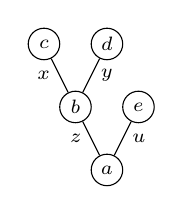
\begin{tikzpicture}[scale=0.8]
        % set up the nodes
        \node (E)[circle,draw=black,minimum size=4mm,inner sep=0.1mm] at (0,0) {\scriptsize $a$};
        \node (F) [circle,draw=black,minimum size=4mm,inner sep=0.1mm] at (-0.5,1) { \scriptsize $b$};
        \node (A) [circle,draw=black,minimum size=4mm,inner sep=0.1mm] at (0.5,1) {\scriptsize $e$};
        \node (Asubt) [circle,draw=black,minimum size=4mm,inner sep=0.1mm] at (-1,2) {\scriptsize  $c$};
        \node (P) [circle,draw=black,minimum size=4mm,inner sep=0.1mm] at (0,2) {\scriptsize $d$};
        % draw arrows and text between them
        \draw[-] (E)--(F) node  [midway,left] {\scriptsize $z$};
        \draw[-] (E)--(A) node  [midway,right] {\scriptsize $u$};
     \draw[-] (F)--(Asubt) node [midway,left] {\scriptsize $x$};
     \draw[-] (F)--(P) node [midway,right] {\scriptsize $y$};
       \end{tikzpicture}}
    
    &&
    \resizebox{2cm}{!}{
    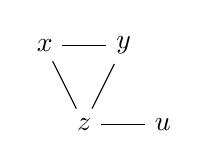
\begin{tikzpicture}
        % set up the nodes
        \node (Z)[] at (-0.5,0) {$z$};
        \node (U)[]  at (0.5,0) {$u$};
        \node (X)[]  at (-1,1) {$x$};
        \node (Y)[]  at (0,1) {$y$};
        % draw arrows and text between them
        \draw[-] (Z)--(U) node  {};
     \draw[-] (Z)--(X) node  {};
     \draw[-] (Z)--(Y) node {};
     \draw[-] (X)--(Y) node {};
       \end{tikzpicture}}
    \end{tabular}
    \end{center}
    \caption{A planar tree with $5$ vertices (left) and its line graph (right).}
    \label{fig:line-graph}
\end{figure}

\subsubsection{Contextual graph-associahedra}
We call \defn{contextual graph-associahedra} the hypergraph polytopes whose underlying hypergraph is a connected simple graph which is moreover contextual.
This family includes all the three previous families, but is far from containing all graph-associahedra.
For instance, we have seen in \cref{non-contextual-2} that the well-known cyclohedra are \emph{not} part of this family. 

\subsubsection{Contextual nestohedra}
We call \defn{contextual nestohedra} the family of hypergraph polytopes whose underlying hypergraph is contextual. 

\begin{rem}
  It would be interesting to characterize combinatorially contextual graphs and hypergraphs.
\end{rem}



\begin{thm}
  \label{thm:examples}
  The following families of hypergraph polytopes are contextual:
  \begin{enumerate}
    \item simplices,
    \item cubes,
    \item associahedra,
    \item permutahedra,
    \item operahedra,
    \item contextual graph-associahedra,
    \item contextual nestohedra.
  \end{enumerate}
\end{thm}

\begin{proof}
  Let us proceed one family at a time.
  \begin{enumerate}
    \item simplices,
    \item We first note that the above description of $\hyper{C}_n$ is saturated, and that $(\hyper{C}_n)_{\set{1,\ldots,m}}=\hyper{C}_m$ (if $m\leq n$).
    So we have to check that  for all $m\leq n$ and all $i,j,k\leq m$, we have $\xyz{k}{{\hyper{H}_n}}{\set{i,j}}$ iff
    $\xyz{k}{{\hyper{H}_m}}{\set{i,j}}$, which follows immediately from the observation that for all $p\geq m$ we have
    $\xyz{k}{{\hyper{H}_p}}{\set{i,j}}$ iff $i<k$ and $j<k$.
    \item associahedra,
    \item permutahedra,
    \item It is proved in~\cite[Lem.~12]{COI} that the connected subsets of $\hyper{G}({\cal T})$ are in bijective correspondence with the subtrees of $\cal T$ having at least two nodes, through a map $E\mapsto  {\cal T}_E$ such that $\hyper{G}({\cal T})_E=\hyper{G}({\cal T_E})$. Suppose, say, that $\set{x,y,z}\inc E$ and $\xyz{x}{\hyper{G}({\cal T})_E}{\set{y},\set{z}}$. Then it means on the tree side that after removing the edge $x$ from ${\cal T}_E$, resulting in two disjoint subtrees ${\cal T}_E^1$ and ${\cal T}_E^2$ of ${\cal T}_E$, we have, say, $y\in{\cal T}_E^1$ and $z\in{\cal T}_E^2$. 
    On the other hand, removing $x$ from ${\cal T}$ results in subtrees ${\cal T}^1$ and ${\cal T}^2$, containing ${\cal T}_E^1$ and ${\cal T}_E^2$, respectively. 
    Therefore $\xyz{x}{\hyper{G}({\cal T}))}{\set{y},\set{z}}$. 
    And vice-versa.
    \item We only need to check that every $2$-dimensional contextual graph-associahedron appears as a $2$-face of a higher dimensional contextual graph-associahedron. 
    \item We only need to check that every $2$-dimensional contextual nestohedron appears as a $2$-face of a higher dimensional contextual nestohedron.
  \end{enumerate}
\end{proof}










%% !TEX root = ../Coherence2.tex

\section{Categorical coherence} 
\label{s:coherence}

%%%%%%%%%%%%%%%%%%%%%%%%%%%%%%%%%%%%%%

\begin{table}[h!]
	\begin{center}
	\begin{tabular}{c|c|c}
	Family & Algebraic structure & Coherence theorem \\
	\hline
	Simplices & - & - \\
	Cubes & - & - \\
	Associahedra & Monoidal category & \cite{MacLane63} \\
	Permutahedra & Categorified permutads & \cite{CLA1} \\
	Operahedra & Categorified operads & \cite{DP15,CLA1} \\
	Contextual graph-associahedra & Categorified reconnectads? & - \\
	Contextual nestohedra & - & - 
	\end{tabular}
	\end{center}
\end{table}

Conjectures: 
\begin{itemize}
  \item contextual graph-associahedra give coherence for (some specific) categorified reconnectads \cite{DotsenkoKeilthyLyskov}
  \item contextual nestohedra give coherence for a hypergraphic generalization
\end{itemize}




\subsection{Interpretation}

Associahedra form a subfamily of operahedra: those obtained from linear trees.  Consider the linear tree

\vspace{-1cm}
\begin{center}
$$\xymatrix @-1.65pc {{\cal L} & = &X \ar @{-}[rr]^{1}&& Y \ar @{-}[rr]^{2}&& Z \ar @{-}[rr]^{3}&& U}
 $$
 \end{center}
 \vspace{-.2cm}
 
 \noindent
 (represented horizontally).  Then $\hyper{G}({\cal L})$ is the associahedron $\hyper{K}^3$. The constructs of
  ${\cal L}$ decorate a pentagon as follows:

%$$
% \xymatrix @-1.65pc {&& 3(2(1)) \ar @{->}[ddll]_{3(\set{1,2})} \ar @{->}[dddrr]^{\set{2,3}(1)}&& \\
% &&&&\\
%3(1(2)) \ar @{->}[dd]^{\set{1,3}(2)} }&&   && \\
% &&&&2(1,3) \ar @{->}[dddll]_{\set{1,2}(3)}\\
%1(3(2)) \ar @{->}[ddrr]^{1(2,3)} &  &\\
% &&&&\\
% &&1(2(3))&&}
%$$
\begin{center}
$$\xymatrix @-1.65pc {&& 3(2(1)) \ar @{->}[ddll]_{3(\set{1,2})} \ar @{->}[dddrr]^{\set{2,3}(1)}&& \\
 &&&&\\
3(1(2))   \ar @{->}[dd]^{\set{1,3}(2)}&&   && \\
 &&&&2(1,3) \ar @{->}[dddll]^{\set{1,2}(3)}\\
 1(3(2)) \ar @{->}[ddrr]^{1(\set{2,3})} &  &\\
 &&&&\\
 &&1(2(3))&&}$$
\end{center}
and are in bijective correspondence with the vertices and edges of Mac Lane's pentagon (cf. Section \ref{preamble-section}). 
  Let us sketch the encoding:
  \begin{itemize}
  \item $(X\otimes_1 Y)\otimes_2 (Z\otimes_3 U)$, where we annotaded the ``compositions'' $\otimes$ with the vertices of $\hyper{K}^3$, can be written $\otimes_2(\otimes_1(X,Y),\otimes_3(Z,U))$ in prefix (or tree) notation. Then we get 
 $2(1,3)$ by removing the leaf nodes of that tree.
 \item $\alpha_{X,Y,Z}\otimes_3 U$ can be interpreted as $(X\otimes_1 Y\otimes_2 Z)\otimes_3 U$ (a non fully parenthesed expression), which likewise 
 translates as $3(\set{1,2})$,where $3(\_)$ makes the job of contextualisation.
 \item Likewise, we can move from
$\alpha_{X,Y\otimes_2 Z,U}$ to $X\otimes_1(Y\otimes_2 Z)\otimes_3 U$ to $\set{1,3}(2)$, where $2$ makes the job of instantiation.
\end{itemize}

Taking the 4-dimensional associahedron $\hyper{K}^5$ (with vertex set $\set{0,1,2,3,4}$), we get the following instance in context of $\hyper{K}^3=\recrestr{\hyper{K}^5}{\set{1,2,3}}$, i.e. of Mac Lane's condition:
\begin{center}
$$\xymatrix @-1.65pc {&& 4(3(2(1(0)))) \ar @{->}[ddll]_{4(3(\set{1,2}(0)))} \ar @{->}[dddrr]^{4(\set{2,3}(1(0)))}&& \\
 &&&&\\
4(3(1(0,2)))  \ar @{->}[dd]^{4(\set{1,3}(0,2))}&&   && \\
 &&&&4(2(1(0),3)) \ar @{->}[dddll]^{4(\set{1,2}(0,3))}\\
 4(1(0,3(2))) \ar @{->}[ddrr]^{4(1(0,\set{2,3}))} &  &\\
 &&&&\\
 &&4(1(0,2(3)))&&}$$
\end{center}
We recover the (encoding of the) edge 
 $$
 \xymatrix @-2pc {&& ((((X_1\otimes_0 X_2)\otimes_1 Y)\otimes_2 Z)\otimes_3 U)\otimes_4 V \ar @{->}[dddddll]_(.6){(\alpha_{(X_1\otimes X_2),Y,Z}\otimes U)\otimes V\quad} && \\
 &&&&\\
 &&&&\\
  &&&&\\
    &&&&\\
( ((X_1\otimes_0 X_2)\otimes_1 (Y\otimes_2 Z))\otimes_3 U)\otimes_4 V  &&   && \\
\ }
$$
displayed of Section \ref{s:introduction} as the top left edge above.


\section{Recovering MacLane}

Let $\hyper{H}$ be a connected hypergraph. 
Suppose that for any connected subset $Y$, and $X \subseteq Y$, the number of connected components of~$\hyper{H}_Y\setminus X$ is less than or equal to $|X|+1$.
Then, we can consider the following variation on \cref{def:signature-hyper}.
Consider the signature $\Sigma_\hyper{H}$ made of the following data: 
\begin{itemize}
  \item Variables are any set $V$. 
  \item Function symbols are pairs of a connected subset of $H$ and one of its subsets 
  $$F:=\{(X,Y) \ | \ X \subseteq Y \subseteq H, \ \hyper{H}_Y \text{ is connected}\}.$$
  \item Sorts are either the ``variable" sort, or a connected subset of $H$, i.e. 
  $$S:=\{ X \subseteq H \ | \ \hyper{H}_X \text{ is connected}\}\cup\{*\}.$$
  \item For $(X,Y) \in F$, we define $\ari(X,Y):=|X|+1$.
  \item All variables $v \in V$ have the same output sort $\outsort(v):=*$, while function symbols $(X,Y) \in F$ have output sort $\outsort(X,Y):=Y$.
  \item For function symbols $(X,Y) \in F$ such that $\hyper{H}_Y,X \leadsto Y_1,\ldots,Y_k$, we define $\insort((X,Y),i):=Y_i$ for $1 \leq i \leq k$, and $\insort((Y,X),i)=*$ for the remaining inputs.
\end{itemize}

Closed terms of output sort $H$ are still in bijection with constructs, i.e. \cref{l:bijection-terms} holds \emph{mutatis mutandis} for this new signature. 
But now one can define rewriting rules that recover precisely MacLane in the case of the associahedra. 








\bigskip

%\emph{Acknowledgements.}   

\bibliographystyle{amsalpha}

\bibliography{Coherence2}


\end{document}



